\documentclass[result.tex]{subfiles}

\begin{document}

    \section*{\centering Theory}

    In this chapter we will formalize the reinforcement learning problem mathematically and define the methods to solve our particular reinforcement learning problem.

    \subsection*{Framework}

    To begin the definition of the reinforcement learning problem we first need to define a few fundamental terms that are required in the following formalization. The basic idea is to learn from interactions in order to achieve a goal. The learner is called the \textit{agent} which interacts with the \textit{environment} by performing \textit{actions} in a sequential manner. The agent is continuously interacting with the environment and it responds based on those interactions in the form of a representation of the \textit{state} of the environment. Not only may the environment change its state, it also give rise to \textit{rewards}, numerical values that the agent is trying to maximize. Figure \ref{fig:agent_env} shows the interactions between the agent and the environment. A complete specification of an environment and how its rewards are determined defines a \textit{task}, which is an instance of a reinforcement learning problem.

    \begin{figure}[H]
        \centering
        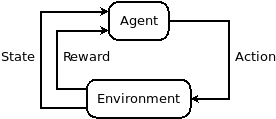
\includegraphics[width=0.6\textwidth]{./images/agent_env}
        \label{fig:agent_env}
        \caption{The agent-environment interaction loop.}
    \end{figure}

    This rather simple framework is actually abstract and flexible enough to be applied in many problems in many different ways. The actions could range from low level controls such as turning the wheels on the car to driving from point A to point B. Similarly, the state could represent current road surface condition to traffic flow in the nearby area. The reward will however always be a single numerical value since we require it to be comparable to be able to determine the best action, the action that will maximize the total amount of reward the agent receives. We will come back to what that means in the following section.

    \subsection*{Markov Decision Process}

    We are going to limit our problem formalization to a special case with discrete time steps, finite state space, finite action space, fully observable state, and episodic tasks. It can be generalized to continuous time steps, infinite state space, infinite action space, partially observable state, and continuing tasks, but it is out of scope for this report.

    \subsubsection*{Notation}

    Before continuing with the definition we need to present the most important notation that will be used from now on through the rest of the report.
    \newline
    $\actionspace$: Action space \\
    $\statespace$: State space \\
    $A_t \in \actionspace$: Action at time $t$ \\
    $S_t \in \statespace$: State at time $t$ \\
    $R_t \in \rewardspace$: Reward at time $t$
    \newline
    where $t \in \{ 0, 1, 2, \ldots, T \}$ since we have discrete time steps. Capital letters with a subscript such as $A_t$ are regarded as random variables while a lowercase letter such as $a$ is a realisation of a random variable.

    \subsubsection*{Dynamics}

    We will now formalize the reinforcement learning problem through the \textit{Markov Decision Process} (MDP), in particular the \textit{finite} MDP, by sticking to the limitations mentioned above. This formalization assumes that the problem satisfies the \textit{Markov property} which means that the one-step dynamics of the problem hold the following

    \begin{align*}
        Pr(S_{t + 1} = \nextstate, R_{t + 1} = r | S_0, A_0, R_1, \ldots, S_{t - 1}, A_{t - 1}, R_t, S_t, A_t) = Pr(S_{t + 1} = \nextstate, R_{t + 1} = r | S_t, A_t),
    \end{align*}

    which in words says that the future state-reward pair is independent of the past actions, states, and rewards given the current action-state pair. That is also equivalent to saying that the current action and state captures all the relevant information from the history. To simplify this formula we write it as

    \begin{align*}
        p(\nextstate, r | s, a) &=
        Pr(S_{t + 1} = \nextstate, R_{t + 1} = r | S_t = s, A_t = a)
    \end{align*}

    and it completely specifies the dynamics of the finite MDP, or equivalently the dynamics of the environment in which the agent is interacting. We can compute anything we might want to get from it such as the the \textit{state-transition probabilities} and the \textit{expected reward} for state-action pairs

    \begin{align*}
        p(\nextstate | s, a) &=
        \sum_r p(\nextstate, r | s, a), \\
        r(s, a) &=
        \expectation \left[ R_{t + 1} | S_t = s, A_t = a \right] =
        \sum_{r \in \rewardspace} r \sum_{\nextstate \in \statespace} p(\nextstate, r | s, a).
    \end{align*}

    \subsubsection*{Policy}

    A \textit{policy} $\pi$ is a distribution over actions given states

    \begin{align*}
        \pi(a | s) &= Pr(A_t = a | S_t = s).
    \end{align*}

    It fully defines the behavior of an agent. It maps an observed state into an action and it could be stochastic in order to enforce \textit{exploration} which we will come back to later. A policy could be as simple as a lookup table or a complicated search process which further makes this framework very flexible.

    \subsubsection*{Reward}

    The \textit{reward signal} is an essential part to learning that will guide the agent to the target behavior. This implies that it is crucial that during the construction of your reinforcement learning problem the underlying reward function that generates the rewards should reflect what you want accomplished. As a simple example, in the game of chess you would consider winning as good and losing as bad and so the reward should reflect that by for instance give +1 reward for winning and -1 reward for losing.

    The sole goal of the agent is the maximize the total reward it receives of the long run so we define the return $G_t$ as

    \begin{align*}
        G_t = R_{t + 1} + \gamma R_{t + 2} + \ldots = \sum_{k = 0}^{\infty} \gamma^k R_{t + k + 1},
    \end{align*}

    where $\gamma \in \left[0, 1 \right]$ is the \textit{discount factor} that determines how much weight the agent should focus on immediate rewards versus future rewards. By adding the discount factor $\gamma < 1$ to $G_t$ we bound it so it does not become $\infty$. The goal of reinforcement learning is to maximize the return $G_t$ but since it is a random variable what we actually do care about is the \textit{state-value function}

    \begin{align*}
        v_{\pi}(s) &= \expectation_\pi \left[ G_t \bigg\rvert S_t = s \right]
        = \sum_a \pi(a | s) \sum_{\nextstate, r} p(\nextstate, r | s, a) \left[ r + \gamma v_\pi(\nextstate) \right]
    \end{align*}

    and the \textit{action-value function}

    \begin{align*}
        q_{\pi}(s, a) = \expectation_\pi \left[ G_t \bigg\rvert S_t = s, A_t = a \right]
        = \sum_{\nextstate, r} p(\nextstate, r | s, a) \left[ r + \gamma \sum_{\nextaction} \pi(\nextaction | \nextstate) q_\pi(\nextstate, \nextaction) \right].
    \end{align*}

    In words these functions expresses the expected return starting from state $s$ and then following policy $\pi$, and the expected return starting from state $s$ and performing action $a$ and then following policy $\pi$ respectively.

    These recursive equations are known as the Bellman equations discovered by Richard Bellman in the 1950s. What we are interested in is finding the Bellman optimality equations

    \begin{align*}
        v_{\ast}(s)
        &= \max_{\pi} v_{\pi}(s) \\
        &= \max_a \sum_{\nextstate, r} p(\nextstate, r | s, a) \left[ r + \gamma v_\ast(\nextstate) \right], \\
        \forall_s v_{\ast}(s) &\geq \forall_{s, \pi} v_{\pi}(s), \\
        q_{\ast}(s, a)
        &= \max_{\pi} q_{\pi}(s, a) \\
        &= \sum_{\nextstate, r} p(\nextstate, r | s, a) \left[ r + \gamma \max_{\nextaction} q_\ast(\nextstate, \nextaction) \right], \\
        \forall_s q_{\ast}(s, a) &\geq \forall_{s, \pi} q_{\pi}(s, a),
    \end{align*}

    and having those makes it trivial to find the optimal policy that maximizes the expected return which is the goal of the agent. It turns out that there always exists such a policy, possibly multiple such policies.

    The optimal policy $\pi_\ast$ is

    \begin{align*}
        \pi_\ast(a | s) &=
        \begin{cases}
            1, & \text{if}\ a = \displaystyle\argmax_{a} q_\ast(s, a) \\
            0, & \text{otherwise}
        \end{cases} \\
        &=
        \begin{cases}
            1, & \text{if}\ a = \displaystyle\argmax_{a} \sum_{\nextstate, r} p(\nextstate, r | s, a) \left[ r + \gamma v_\ast(\nextstate) \right] \\
            0, & \text{otherwise},
        \end{cases} \\
    \end{align*}

    and we can clearly see that is it easier to acquire the optimal policy if we have access to the optimal action-value function. The problem is that there are, in general, no closed form solution to finding these optimal value functions and so there in the difficulty of reinforcement learning. After a short explanation of exploration and the problem we will present a few iterative solution methods for finding these optimal value functions, the action-value function in particular, that have been used in this report.

    \subsubsection*{Exploration versus Exploitation}

    An important concept in reinforcement learning is the \textit{exploration-exploitation} trade-off. It refers to the problem that the agent does not know how it should behave to maximize the expected return and thus have to interact with the environment to learn by trial-and-error. This means that it has to explore the environment by interactions and observe their consequences and the reward signals. This information does not contain what the \enquote{right} action was supposed to be but the agent can still construct a policy from it. Exploting means that the agent is using its current policy to determine the best action, i.e., is greedy with respect to the policy. It can happen that the current policy is stuck in a local optima because the agent has not explored the search space thorough enough to build a good estimate of the other action performances.

    A simple technique to enforcing exploration is by training using $\epsilon$-greedy policy that take the greedy action with probability $1 - \epsilon$ and a uniformly random action with probability $\epsilon$. This is the approach taken in this report but there are more sophisticated techniques to balance these two acts.

    \begin{algorithm}[H]
        \caption{$\epsilon$-Greedy Policy}
        \label{alg:epslion-greedy-policy}
        \begin{algorithmic}[1]
            \Require{State $s$, Action-value function $q$,
            Exploration rate $\epsilon \in [0, 1]$}
            \Statex
            \Function{EpsilonGreedyPolicy}{$s, q, \epsilon$}
            \Let{sample $u \sim U(0, 1)$}
            \If{$u < \epsilon$}
            \Let{sample $i \sim U(\{ 1, 2, \ldots, |\actionspace| \})$}
            \Let{$a = \actionspace_i$}
            \Else
            \Let{$a = \displaystyle\argmax_a q(s, a)$}
            \EndIf
            \State
            \Return{$a$}
            \EndFunction
        \end{algorithmic}
    \end{algorithm}

    \subsection*{Snake}

    This report is meant to look at some of the fundamental building blocks of reinforcement learning and in order to do so we need a problem that we would like to solve. Snake is an old game\footnote{https://en.wikipedia.org/wiki/Snake\_(video\_game)} and has been around for a long time and there are many variations of it. In this report, the game is played out as simple as possible with only one player, i.e., the agent and no obstructing environment. The goal of the game is that you play as a snake by controlling the head and the aim is to eat as many apples as possible without colliding with either the snake's body or the edges of the game board. The difficulty is that each time you eat an apple your body becomes longer and thus larger portion of the game board is covered by it. In order to reduce the state space the game board is played on a 5x5 grid which can be seen in figure \ref{fig:snake}.

    \begin{figure}[H]
        \centering
        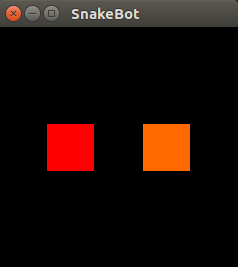
\includegraphics[width=.3\textwidth]{./images/snake1}\hfill
        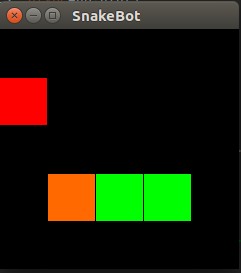
\includegraphics[width=.3\textwidth]{./images/snake2}\hfill
        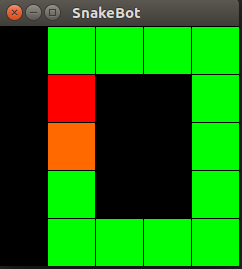
\includegraphics[width=.3\textwidth]{./images/snake3}
        \label{fig:snake}
        \caption{5x5 board of Snake where the snake consists of the orange (head) and green parts (body) and the red part is the apple.}
    \end{figure}

    A term that was mentioned previously was \textit{episodic task} which refers to problems that have a natural notion of final time step which Snake does, that is when the snake collides with something. We denote this state as the \textit{terminal state} which will follow with a reset of the game in the same starting state independently of how it ended.

    \subsubsection*{MDP}

    With the previous formalization of the MDP we can now define Snake's MDP and its a rather simple definition. We assume that the actions are completely deterministic and the state transitions are also deterministic. Given our action space, $\actionspace = \{ \text{North}, \text{South}, \text{West}, \text{East} \}$, that means that if the snake moves north it will move north, not any other direction, and the next state will reflect that. Figure \ref{fig:snake} shows three different states that the agent will be able to observe completely. There is no stochasticity in the environment except the positioning of the apple which will be randomly placed uniformly whenever eaten so only one food source at any single point in time. We have chosen that each eaten apple gives the player 10 game points and at the end of the game the total score is thus 10 $\times$ number of apples eaten.

    \subsection*{Temporal Difference Learning}

    \textit{Temporal Difference} (TD) learning is a learning methodology that learns directly from raw experience without a model of the environment's dynamics. It update new estimates partially on previous estimates without waiting for the final outcome, i.e. bootstraps estimates. The algorithms, or learning methods, that have been used in this paper are all based on TD learning and will be described below.

    \subsubsection*{Q-Learning}

    Q-learning is a widely used algorithm that was developed by \textbf{(Watkins, 1989)} and is heavily used to day combined with the emergence of neural networks \textbf{deep reinforcement learning, atari}. It is defined as

    \begin{align*}
        Q(S_t, A_t) &=
        Q(S_t , A_t) +
        \alpha \left[
        R_{t + 1} +
        \gamma \max_a Q(S_{t + 1}, a) - Q(S_t, A_t).
        \right]
    \end{align*}

    It is a so called \textit{off-policy} method which is indicated by the $\max_a$ operation. That means it uses a greedy algorithm to estimate the return at the next step rather than following its current policy, therefore is off its own policy. The Sarsa algorithm described below is an example of a on-policy method.

    \subsubsection*{Sarsa}

    \begin{align*}
        Q(S_t, A_t) &=
        Q(S_t , A_t) +
        \alpha \left[
        R_{t + 1} +
        \gamma Q(S_{t + 1}, A_{t + 1}) - Q(S_t, A_t)
        \right]
    \end{align*}

    \subsubsection*{Expected Sarsa}

    \begin{align*}
        Q(S_t, A_t) &=
        Q(S_t , A_t) +
        \alpha \left[
        R_{t + 1} +
        \gamma \mathbb{E} \left[ Q(S_{t + 1}, A_{t + 1}) | S_{t + 1}
        \right] -
        Q(S_t, A_t)
        \right] \\
        &=
        Q(S_t , A_t) +
        \alpha \left[
        R_{t + 1} +
        \gamma \sum_a \pi (a | S_{t + 1}) Q(S_{t + 1}, a) -
        Q(S_t, A_t)
        \right]
    \end{align*}

    \subsection*{Other Learning Methods}

    \subsubsection*{Dynamic Programming}

    \subsubsection*{Monte Carlo}

    \subsubsection*{Extensions}

\end{document}
